
%NOTE: to be used with \usepackage{subfiles} in the main file.
%Subfiles go in folders which live with the main file.
%Bibliography and preamble go in the main file.

%%%%%%%%%%%%%%%%%%%%%%%% PREAMBLE %%%%%%%%%%%%%%%%%%%%%%%%
\providecommand{\main}{..}

\documentclass[main]{subfiles} %Each instance of `../' elevates one folder to find the main file

\begin{document}

%%%%%%%%%%%%%%%%%%%%%%% DOCUMENT %%%%%%%%%%%%%%%%%%%%%%%

% \tableofcontents % Can be useful to load a TOC while writing

\doublespacing

\schapter{Sample generation and machine learning techniques}

\hypsection{Generation of signal and background events}
\label{sect:event-generation-chain}
\vspace{20pt}

The Monte Carlo samples used in the analysis are produced using a generation chain with multiple steps involving different software. Both signal and background event generation consist of the same steps. However, both samples are produced separately in order to obtain the respective signal and background datasets. Two signal processes will be considered, the first one is used to study the tagging of boosted top quarks and the second one to study the tagging of boosted $W$ bosons. These signal samples will be used together with a single QCD background sample of light quarks and gluons, taking into account the discussion of section \ref{sect:substructure}.\\

The generation chain begins with the generation of matrix elements at leading order (LO) in QCD and electroweak couplings using \textsc{MadGraph5\_aMC@NLO} v2.9.12 \cite{Alwall2014} with the \textsc{NN23LO1} PDF set \cite{Ball2017}. The process defined to produce the signal top jets consists of top quarks decaying in the entirely hadronic channel $pp \rightarrow t \tilde{t}$, ($t \rightarrow W^+ b$, $W^+ \rightarrow jj$), ($\tilde{t} \rightarrow W^- \tilde{b}$, $W^- \rightarrow jj$). On the other hand, the process used to produce the background sample is the default QCD dijet production routine $pp \rightarrow jj$ where the $j$ jets are composed of light quarks ($b$'s included) and gluons.\\

The Feynman diagrams of the processes used to generate the matrix elements for the boosted top quark signal events are shown in figure \ref{fig:feynman_tt}. These correspond to the production of top quark-antiquark ($t\bar{t}$) pairs through strong interactions. These kind of interactions are mediated by gluons ($g$), which are massless particles that interact with quarks, antiquarks and other gluons by means of the colour charge (see section \ref{sect:jets_algorithms}). It should be noted, however, that single top quark production is also possible through weak interactions. Nonetheless, at the LHC top quarks are predominantly produced in ($t\bar{t}$) pairs \cite{deJong2009}. Consequently, the processes selected for this study correspond to this kind of production. \\


\begin{figure}[H]
     \centering
     \begin{subfigure}[h]{0.49\textwidth}
         \centering
         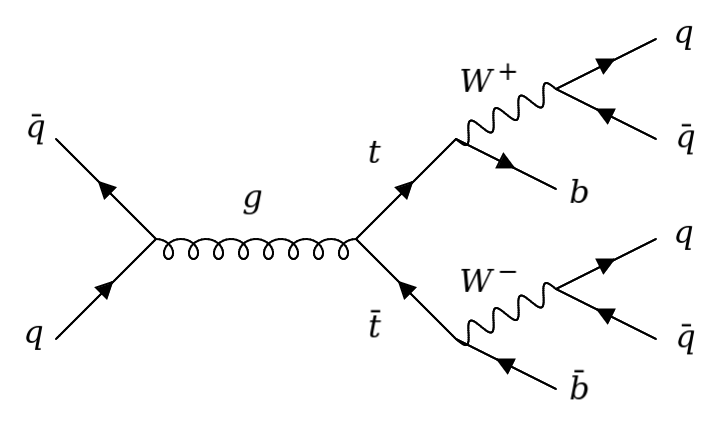
\includegraphics[width=0.8\textwidth]{../Figures/Datasets/pp_tt/qq_tt_qq.png}
          \caption{}
         \label{fig:feynman_tt_qqanihilation}
     \end{subfigure}
     \begin{subfigure}[h]{0.49\textwidth}
         \centering
         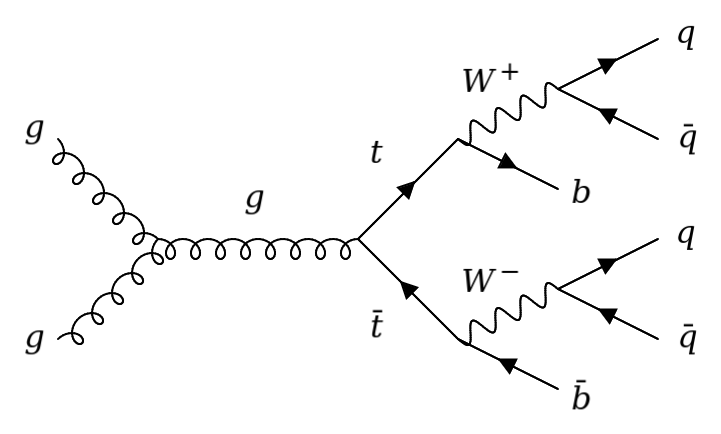
\includegraphics[width=0.8\textwidth]{../Figures/Datasets/pp_tt/gg_tt_qq_1.png}
          \caption{}
         \label{fig:feynman_tt_ggfusion1}
     \end{subfigure}
     \par\bigskip
     \begin{subfigure}[h]{0.49\textwidth}
         \centering
         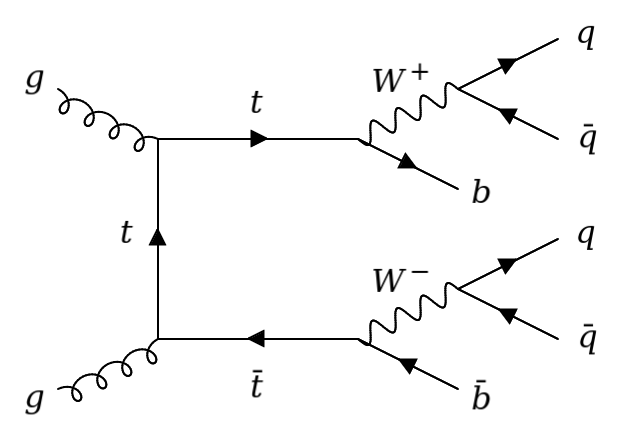
\includegraphics[width=0.8\textwidth]{../Figures/Datasets/pp_tt/gg_tt_qq_2.png}
          \caption{}
         \label{fig:feynman_tt_ggfusion2}
     \end{subfigure}
     \begin{subfigure}[h]{0.49\textwidth}
         \centering
         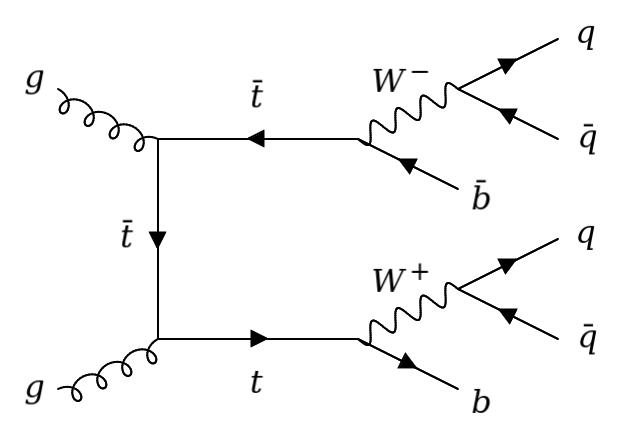
\includegraphics[width=0.8\textwidth]{../Figures/Datasets/pp_tt/gg_tt_qq_3.png}
          \caption{}
         \label{fig:feynman_tt_ggfusion3}
     \end{subfigure}
     \caption{Feynman diagrams of the signal processes used for the simulation of boosted top quark production via (a) quark pair annihilation and (b) - (d) gluon fusion.}
        \label{fig:feynman_tt}
\end{figure}

Regarding the ($t\bar{t}$) pair production, two main methods are considered. The first one is the annihilation of a quark with its antiquark, which produces a gluon that afterwards originates a ($t\bar{t}$) pair. The second method of production is gluon-gluon fusion, in which two gluons decay into a ($t\bar{t}$) pair. Although quark-antiquark annihilation was the method which originated most top quarks when the top quark was first discovered at Tevatron in 1995, gluon-gluon fusion dominates at high-energy pp collisions and corresponds to 90\% of the top quark production at the LHC \cite{Quadt2006}. \\

After the top quarks are produced, they decay almost exclusively into a $W$ boson and a $b$ quark. $W$ bosons are the mediators of charged currents in weak interactions, and as such, they couple to both quarks and leptons. Therefore $W$ bosons can decay into a charged lepton and neutrino pair or into a quark-antiquark pair with a difference in charge of 1 or -1, namely a top-type quark(antiquark) and a down-type antiquark(quark). The fully hadronic channel of the ($t\bar{t}$) production processes is achieved when the $W$ bosons decay into a quark-antiquark pair (see figure \ref{fig:feynman_tt}). \\

The fully hadronic decay channel has the largest signal yield compared to the channels where $W$ bosons decay into leptons (either just one or both of them) \cite{Silva2013}. However, having only jets in the final state, this channel is dominated by the large QCD multijet background present at the LHC. As was stated previously, this is the reason for which being able to identify boosted particles in this channel by using jet substructure techniques is so interesting. When boosted to a high enough energy the large R jets originated by top quarks will have a substructure corresponding to the three lobes of energy mentioned in \ref{sect:substructure}, one coming from the $b$ quark and the other two coming from the $W$ boson. \\

After the amplitudes and mappings for the relevant processes have been obtained they are passed to \textsc{MadEvent} \cite{Maltoni2003}, which generates the unweighted tree-level Les Houches events. Both signal and background datasets consist of 500000 events generated at a centre-of-mass energy of 14\;TeV. During the event generation stage, a parton-level momentum phase space cut is implemented on all partons in order to reduce the computing time for the simulations. Only boosted particles are of interest for this study, and the parton-level cut allows more fat jets to be produced in the established number of events. The cut used is $p_T > 350$\;GeV and it applies at parton-level to both gluons and light quarks, as well as $W$ bosons and top quarks. \\

% \textbf{This initial $p_T$ cut value is later increased for subsequent analyses.}\\

The tree-level events are showered using \textsc{Pythia} v8.306 \cite{Sjostrand2015} with the default settings proposed in the \textsc{MadGraph5}'s implementation of \textsc{Pythia 8} in order to obtain hadron-level events in \textsc{HEPMC} format \cite{Dobbs2001}. Subsequently, the detector response is simulated via \textsc{Delphes} v3.5.0 \cite{deFavereau2014} using the default ATLAS detector configuration card with the inclusion of the fat jet reconstruction module provided by the \textsc{FastJet} v3.3.4 library \cite{Cacciari2012}.\\

The fat jets used in the analysis are reconstructed via \textsc{FastJet} using the anti-$k_T$ algorithm with $R =$ 1.0. The $\tau_N$ values associated to each fat jet are computed from the three-momenta of $N$ candidate subjets using the $N$-subjettiness package (v2.2.6) of the \textsc{FastJet} contrib v1.051. In order to obtain the candidate subjets needed for the $\tau_N$ computations the fat jet is reclustered with an exclusive $k_T$ algorithm \cite{Khelifa-Kerfa2022}. \\

% \textbf{(this radius parameter is later increased for subsequent analyses)}

At high luminosity hadron colliders such as the LHC, the presence of pile-up energy and the underlying event interferes in analyses involving large $R$ jets because they lead to soft, wide-angle contaminations which lead to the dilution of the jet substructure. Grooming techniques are useful to remove these contaminations. The grooming methods applied to the jets reconstructed in this analysis are trimming \cite{Krohn2010}, pruning \cite{Ellis2009} and soft-dropping \cite{Larkoski2014} algorithms. These methods are implemented via \textsc{FastJet} integration, using the default parameters in the ATLAS configuration card of \textsc{Delphes 3}. This selection of parameters is done based on various studies that have been carried out previously in order to compare and optimize the performance of the different methods.\\

It should be noted that the description of the event generation process described above also applies for the generation of the signal sample used to study the tagging of boosted $W$ bosons. In this case the process used for the tree-level event generation is $W$ pair production, with each $W$ decaying in the full hadronic channel $pp \rightarrow W^{+}W^{-}$, ($W^{+} \rightarrow jj$), ($W^{-} \rightarrow jj$), where the $j$ jets are defined as in the process used in the background sample generation. The feynman diagrams of the processes used for the boosted $W$ signal events are shown in figure \ref{fig:feynman_WW}. The discussion about the $W$ bosons decaying into a quark-antiquark pair in the full hadronic channel carried out for the boosted top signal is also valid in this case. However, the large R jets resulting from the boosted $W$ bosons will have two lobes of energy, associated with the quark-antiquark pair that they decay into. \\

\begin{figure}[H]
     \centering
     \begin{subfigure}[h]{0.49\textwidth}
         \centering
         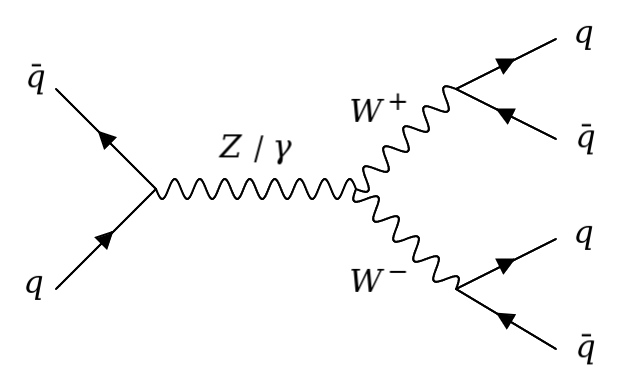
\includegraphics[width=0.8\textwidth]{../Figures/Datasets/pp_WW/qq_aZ_WW_qq.png}
          \caption{}
         \label{fig:feynman_WW_qqanihilation1}
     \end{subfigure}
     \begin{subfigure}[h]{0.49\textwidth}
         \centering
         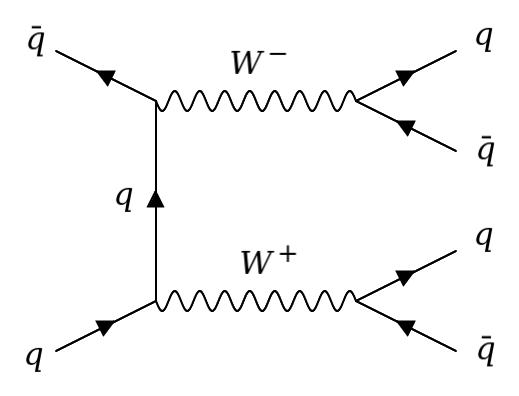
\includegraphics[width=0.8\textwidth]{../Figures/Datasets/pp_WW/qq_WW_qq.png}
          \caption{}
         \label{fig:feynman_WW_qqanihilation2}
     \end{subfigure}
     \caption{Feynman diagrams of the signal processes used for the simulation of boosted $W$ production.}
        \label{fig:feynman_WW}
\end{figure} 

\vspace{11pt}

\hypsection{Machine learning implementation}
\vspace{20pt}

The discrimination between signal and background events can be initially done as a cut based analysis by applying subsequent cuts on the substructure variables proposed earlier. This can be easily seen from the comparison between signal and background distributions of the jet mass and $\tau_{N+1}/\tau_N$ variables (see section \ref{sect:results}). However, in previous studies this kind of cut based selections have been found to be insufficient when dealing with data similar to that of this work \cite{Li2016}. With that in mind, the tagging method proposed in this study will be based on machine learning techniques, which take an increasingly important role in LHC experiments as time passes, specially in the field of jet tagging \cite{Cagnotta2022}.  \\

The machine learning aspect of the proposed tagging method consists on the use of multivariate analysis algorithms. Initially, multiple multivariate classifiers will be considered and their performance will be compared. The classifiers being evaluated are the k-nearest neighbour classifier (k-NN), linear discriminant analysis (LD), function discriminant analysis (FDA), 1-dimensional likelihood estimator (with and without PCA-transformed input variables), Friedman's RuleFit method (RuleFit), multilayer perceptron artificial neural network (MLP), boosted decision tree (BDT) and a deep learning neural network (DNN). For more information on each one of these methods see ref. \cite{Hoecker2009}.\\

The different multivariate methods are implemented using the \textsc{Toolkit for Multivariate Data Analysis with ROOT (\textsc{TMVA 4})} \cite{Hoecker2009}. This toolkit, integrated into the \textsc{ROOT} analysis framework \cite{Brun1997} allows for the training, testing, performance evaluation and application of the different multivariate classification algorithms. The multivariate techniques used belong to the family of "supervised learning" algorithms. They use a training set of events for which the desired output is known (i.e. the algorithm knows if the event is a signal or a background event) in order to determine the mapping function that describes the decision boundary used during the classification. \\

As will be discussed in section \ref{sect:results}, the classifier which achieved the best performance when dealing with both kind of signal fat jets, and therefore was selected to carry on with the proposed tagging method was the boosted decision tree (BDT). A decision tree is a binary tree structured classifier in which yes/no type decisions about a particular variable are repeatedly taken until certain stop criterion is met \cite{Quinlan1987}. By doing so, the phase space is divided into multiple regions which are subsequently categorized as either signal or background, depending on the type of the majority of training events that remain after the last node is reached. On another hand, the \textit{boosting} of a multivariate classifier refers to the enhancement of its performance and its stability with respect to statistical fluctuations in the training sample by applying the method successively to reweigthed versions of the training data. In the case of a boosted decision tree, this implies the use of multiple trees which form a \textit{forest}, which is afterwards merged into a single classifier. \\

In addition to the BDT, the results of using a deep neural network (DNN) as the classification mechanism are also taken into account. A neural network is a type of machine learning model inspired by the structure and function of human brains. A DNN is composed of multiple (hence the "deep") layers of interconnected nodes called neurons which process and transmit data. The DNN uses the training dataset to adjust the weights and biases of its neurons and their connections by iteratively computing the difference between its predicted outputs and the true event type (whether signal or background), using a technique called backpropagation. This iterative process minimizes a defined loss function and aims to improve the DNN's ability to correctly classify the data. \\

The discriminating variables used as input for the different classifier algorithms are the fat jet mass and $N$-subjettiness, which contain information on the substructure of the fat jets. As it was mentioned before, the $\tau_N$ variables do not have much discriminant power by themselves, but rather their ratios do. An advantage of the multivariate classifiers is that they can be supplied with a full set of $\tau_N$ variables so that more complex relations between them can be taken into account when defining the decision boundary that optimizes the classification. As the number of $\tau_N$ variables used as input increases, so does the information that the algorithm can use to carry out the classification. However, it is expected that for higher $N$ values, $\tau_N$ won't contribute as much to the discrimination. Therefore the performance with different number of $\tau_N$ variables used as input will be considered. \\

The training and testing sets of events are randomly selected from the generated signal and background samples. For both signal and background samples, half of the events are assigned to the training dataset and the other half are assigned to the testing dataset so that they both have the same size. Lastly, it is worth mentioning that for all the multivariate methods, the default configuration of the classifier algorithms in \textsc{TMVA} is used. 




















% \bibliographystyle{../../PhilReview} %%bib style found in bst folder, in bibtex folder, in texmf folder.
% \nobibliography{Zotero} %%bib database found in bib folder, in bibtex folder
% \nobibliography{../../Thesis_bib}
\biblio

\end{document}
